% Nature Communications
% https://www.nature.com/ncomms/submit/how-to-submit
% https://mts-ncomms.nature.com/cgi-bin/main.plex
%
% sn-article.cls (Springer Nature 통합 공식 템플릿) 권장
% 공식 다운로드 페이지 (Springer Nature Author Services)
% https://www.springernature.com/gp/authors/campaigns/latex-author-support
% 직접 템플릿 ZIP 다운로드
% https://media.springernature.com/full/springer-cms/rest/v1/content/19238648/data/v7
%
%
% 최종 제목	Hierarchical Memory Orchestration Enables Scalable and Efficient Large Language Model Inference
% 시스템 명칭	MBALL (Memory-Balanced Adaptive Layered Loader)
% 투고 저널	Nature Communications
% 적정 분량	10–12 pages / 5,000–6,500 words
% 수정 강도	중간 (프레이밍 중심, 구조 유지)

%
% 다운로드 주소(Overleaf)
% https://www.overleaf.com/latex/templates/springer-nature-latex-template/myxmhdsbzkyd



%%---------------- IEEEtran template: start ------------------

% \documentclass[9pt,technote]{IEEEtran}
% \documentclass[journal,10pt,onecolumn,draftclsnofoot,]{IEEEtran}
%\documentclass[10pt,journal,onecolumn]{IEEEtran}
%\documentclass[10pt,journal]{IEEEtran}
%\documentclass[journal]{IEEEtran}
\documentclass[10pt,conference]{IEEEtran}

\IEEEoverridecommandlockouts
% The preceding line is only needed to identify funding in the first footnote. 
% If that is unneeded, please comment it out.
\usepackage{cite}
\usepackage{amsmath,amssymb,amsfonts}
\usepackage{graphicx}
\usepackage{textcomp}
\usepackage{ifthen}


\usepackage{doi}

% ----- Minimal-Consistent experiment reporting helpers -----
\newcommand{\ntrials}{5}
\newcommand{\ci}{95\%~CI}
\newcommand{\hwsetup}{2~$\times$~NVIDIA~A100~(80GB), 512GB DRAM, NVMe~Gen4}
\newcommand{\swsetup}{PyTorch~2.4, CUDA~12.2, vLLM~\cite{kwon2023pagedattention}~0.5.3}
\newcommand{\capinfo}{\emph{Means across $n=\ntrials$ runs (\ci). HW: \hwsetup; SW: \swsetup.}}
% -----------------------------------------------------------

%%---------------- IEEEtran template: end  ------------------- 

%% ------------- ORC ID Template: Start ----------------------
% https://tex.stackexchange.com/questions/498688/orcid-in-latex-file-of-ieee-trans-in-a-customized-position

\usepackage{scalerel}
\usepackage{tikz}
\usetikzlibrary{svg.path}

\definecolor{orcidlogocol}{HTML}{A6CE39}
\tikzset{
  orcidlogo/.pic={
    \fill[orcidlogocol] svg{M256,128c0,70.7-57.3,128-128,128C57.3,256,0,198.7,0,128C0,57.3,57.3,0,128,0C198.7,0,256,57.3,256,128z};
    \fill[white] svg{M86.3,186.2H70.9V79.1h15.4v48.4V186.2z}
                 svg{M108.9,79.1h41.6c39.6,0,57,28.3,57,53.6c0,27.5-21.5,53.6-56.8,53.6h-41.8V79.1z M124.3,172.4h24.5c34.9,0,42.9-26.5,42.9-39.7c0-21.5-13.7-39.7-43.7-39.7h-23.7V172.4z}
                 svg{M88.7,56.8c0,5.5-4.5,10.1-10.1,10.1c-5.6,0-10.1-4.6-10.1-10.1c0-5.6,4.5-10.1,10.1-10.1C84.2,46.7,88.7,51.3,88.7,56.8z};
  }
}

\newcommand\orcidicon[1]{\href{https://orcid.org/#1}{\mbox{\scalerel*{

\begin{tikzpicture}[yscale=-1,transform shape]
\pic{orcidlogo};
\end{tikzpicture}
}{|}}}}

%% ------------- ORC ID Template: End ----------------------


 
%% ------------- Geunsik Area : Start ----------------------



% How to hide statements: 
%   - To enable  tags: \iftrue  and \fi
%   - To disable tags: \iffalse and \fi
% How to turn-on (or turn-off) page number:
%   - To turn-on  the page number: {plain}
%   - To turn-off the page number: {empty}
% Usage (Syntax): 
%   \documentstyle[twocolumn]{article}
%   \pagestyle{empty}
%    ...
%   \maketitle
%   \thispagestyle{empty}

% How to print the page number at each page 
%\pagestyle{empty}


% How to support Korean language with the 'latexmkrc' file in www.overleaf.com
% \usepackage{kotex}  % commented for IEEE camera-ready (English)

% How to separate languages (e.g., ko, en) for paper writing
\usepackage{ifthen} % 조건문 사용
\newcommand{\lang}{en} % ko 또는 en 으로 설정


% 상단 메뉴에서 Menu → Compiler → XeLaTeX (또는 LuaLaTeX) 으로 변경하세요.
% \usepackage{fontspec}
% Overleaf에서 IEEEtran.cls + pdfLaTeX → 기본은 Computer Modern
% IEEE 최종 PDF (출판 버전) → Times New Roman (Times 계열)
% 
%\ifthenelse{\equal{\lang}{ko}}{
%  \setmainhangulfont{NanumGothic}
%}{\setmainfont{Times New Roman}
%}




% 익명 처리 여부 (1 = 실명, 0 = 익명)
\newcommand{\anonymous}{1}

%% To keep strictly tuned whitespace rules among section (e.g., section, subsection, and subsubsection)
%% for decreasing or increasing the vertical space between section
\usepackage{titlesec}
\titlespacing*{\section}{0.80pt}{0.50\baselineskip}{0.20\baselineskip}
\titlespacing*{\subsection}{0.80pt}{0.50\baselineskip}{0.20\baselineskip}
\titlespacing*{\subsubsection}{0.80pt}{0.50\baselineskip}{0.20\baselineskip}

%% Reduce vertical space (padding) after figure (a big effect)
%% Warning: "Text page 7 contains only floats."
%% https://www.reddit.com/r/LaTeX/comments/b4mipa/how_to_decrease_space_between_paragraph_and/
\setlength{\textfloatsep}{0.60pt}
\setlength{\abovecaptionskip}{0.60pt}
\setlength{\belowcaptionskip}{0.60pt}


% How to print date, hour, and minute to maintain the current version of the paper.
% Append the below statement in the 'abstract' section.
% For example, write "[Notice] This document was compiled on: \today\ at \currenttime." 
\usepackage[short,nodayofweek,level,24hr]{datetime}


% for pseudo code
\usepackage{algorithm}
\usepackage[noend]{algpseudocode}

% # for using a number symbol (\ding{3})
\usepackage{pifont}

% Text highlight and color (e.g. \hl, \textcolor )
\usepackage{xcolor,color,soul}
%\usepackage{soul}

% Hyperlinks to content
%\usepackage[linktocpage=true]{hyperref}
%\usepackage{hyperref}
%\usepackage[hidelinks]{hyperref}


\usepackage{xcolor} % 색상 지원
\usepackage{hyperref}

\hypersetup{
    colorlinks=true,
    linkcolor=red,   % table, figure, equation, section
    citecolor=red,   % citation
    urlcolor=red     % URL
}



% How to support a code listing
\usepackage{listings}

% set the default code style
\lstset{
    frame=tb, % draw a frame at the top and bottom of the code block
    tabsize=4, % tab space width
    showstringspaces=false, % don't mark spaces in strings
    numbers=left, % display line numbers on the left
    commentstyle=\color{green}, % comment color
    keywordstyle=\color{blue}, % keyword color
    stringstyle=\color{red} % string color
}

% makecell
\usepackage{makecell}
\usepackage{tabu}

\usepackage{tabularx}  % 가로 폭 자동 조절 패키지
\usepackage{makecell}  % 줄바꿈 지원
\usepackage{booktabs}  % 더 깔끔한 표 선 (논문용)

\usepackage{float}
\usepackage[numbers,sort&compress]{natbib}

%% ------------- Geunsik Area : End --------------------------



%% ----------------- Document area: start --------------------
% Modify edit the below statements for your paper.

\usepackage{placeins}
\usepackage{dblfloatfix}

%---- Float placement tuning (reduce whitespace in two-column layout)
\setcounter{topnumber}{2}
\setcounter{bottomnumber}{2}
\setcounter{totalnumber}{4}
\renewcommand{\topfraction}{0.92}
\renewcommand{\bottomfraction}{0.92}
\renewcommand{\textfraction}{0.06}
\renewcommand{\floatpagefraction}{0.86}
\renewcommand{\dbltopfraction}{0.92}
\renewcommand{\dblfloatpagefraction}{0.86}
\flushbottom

\begin{document}
% \tableofcontents

%\title{MBALL: Theoretical and Empirical Analysis of Memory Ballooning for LLM Serving}
%\title{Theoretical and Empirical Analysis of Memory Ballooning for LLM Serving}
%\title{Toward Cost-Efficient LLM Serving: A System-Level Memory Optimization Approach}
%\title{ORION: Hierarchical Memory Orchestration for Scalable Large Language Model Inference}
%\title{ORION: regime-aware orchestration of hierarchical memory systems for scalable AI inference
%\title{Regime-dependent principles of hierarchical memory orchestration for large-model inference}
%\title{Phase transitions in hierarchical memory systems governing large-scale model inference}
%\title{Hierarchical memory orchestration reveals regime-dependent limits in large-scale model inference}
\title{Regime-dependent limits of hierarchical memory orchestration in large-scale AI inference}
\input{./section/005_author.tex}
\begin{abstract}
As artificial intelligence models scale beyond fast-memory capacity, inference latency is increasingly governed by coordination across hierarchical memory systems rather than computation alone. This is especially acute in industrial cyber--physical systems (CPS), where inference must be not merely fast on average but deterministically bounded within PLC scan cycles and TSN time windows. Here we show that such coordination is not continuously optimizable, but instead exhibits intrinsic, regime-dependent limits. We decompose end-to-end latency into four components---compute, locality, inter-tier transfer, and synchronization---and identify three operational regimes---capacity-limited, coordination-dominated, and I/O-limited---defined by two dimensionless ratios: the capacity ratio $\alpha$ and the I/O pressure ratio $\beta$. Transitions between regimes are abrupt rather than gradual.

Using a minimal multi-tier transfer model, we derive analytically interpretable regime boundaries that explain why orchestration strategies effective in coordination-dominated regimes fail predictably once capacity or bandwidth limits are crossed. We build ORION (previously RAMSES), a lightweight orchestrator that coordinates GPU VRAM, host DRAM, and NVMe under regime-aware control. On industrial language and vision workloads, ORION reduces model load time by up to 60\%, inference latency by 35\%, and peak VRAM usage by 15\%, while improving throughput per watt by 18.5\%. Performance remained stable through 72 hours of stress testing, with out-of-SLA yield falling almost tenfold. The timing violation rate of $P_{\mathrm{timing}} = 0.004$ clears IEC~61508 SIL-2, connecting regime-aware memory orchestration to industrial safety compliance. Together, these results establish regime-dependent orchestration as a general principle for memory-bound AI inference and other hierarchical-memory systems, showing that hierarchical memory coordination is regime-dependent in a way that can be written down formally---and once it is, the engineering problem becomes tractable. The analysis reframes optimization as a problem of regime-aware design rather than continuous tuning, and the boundary values we derive give system designers concrete targets for stable, energy-efficient inference within industrial information-system stacks.
\end{abstract}


\begin{IEEEkeywords}
Large Language Models, Memory Optimization, Latency Reduction, GPU Resource Management, System Framework
\end{IEEEkeywords}






% [moved:fig:regime_map]



%------------------------------------------------------------

% [moved:fig:consolidated]



%------------------------------------------------------------

% [moved:tab:cross-model]


%-------------------------------------------------------------------

% [moved:tab:energy]


%-----------------------------------------------------------


% [moved:tab:regime_guidelines]



%-----------------------------------------------------------------


% [moved:tab:baseline_comparison]


%---------------------------------------------------------------------

% [moved:tab:ablation]



%------------------------------------------------------------------------

% [moved:tab:multi_gpu]



%----------------------------------------------------------------------


% [moved:fig:orion_overview]




%====================
% Unplaced materials (no reference found)
%====================

% [moved:fig:regime_map]


% [moved:fig:consolidated]


% [moved:tab:cross-model]


% [moved:tab:energy]


% [moved:tab:ablation]


\section{Introduction}
\label{sec:introduction}

Modern foundation models have shifted the performance frontier of AI inference
from arithmetic throughput to \emph{data coordination}.
When model weights, activations, and key--value (KV) caches exceed accelerator
memory, inference latency is governed less by compute and more by how efficiently
execution coordinates data movement across a hierarchical memory system spanning
device memory, host memory, and secondary storage~\cite{ma2026inference,gholami2024memorywall}.

This shift carries pressing economic and environmental stakes.
Once a model is trained, the recurring cost of \emph{serving} it dominates its
lifetime resource footprint.
Hardware analyses identify memory capacity, memory bandwidth, and interconnect
latency---not arithmetic throughput---as the binding constraints of the inference
phase~\cite{zhou2024survey}.
These constraints translate into macro-level exposure: aggregate capital
expenditure across major hyperscalers is on track to overtake operating cash
inflows by end of 2026~\cite{juniewicz2026hyperscaler}, and AI infrastructure
is absorbing available memory supply faster than it can be
produced~\cite{chey2026tpd}.
In this context, characterizing the \emph{intrinsic limits} of memory
orchestration is not merely a systems-optimization concern but a prerequisite
for the financial and energy viability of inference-driven AI.

A large body of systems work reduces memory pressure via CPU/NVMe offloading
and heterogeneous execution~\cite{flexgen2023,aminabadi2022deepspeedinference},
smart GPU--CPU swapping~\cite{huang2020swapadvisor}, and KV-cache management
for long-context batching~\cite{kwon2023pagedattention}.
These techniques deliver substantial gains in some configurations yet show
diminishing returns---or even performance inversion---in others.
This variability raises a fundamental question that incremental optimization
studies do not answer: \emph{Is hierarchical memory orchestration a continuously
optimizable engineering problem, or does it admit intrinsic boundaries beyond
which additional coordination cannot improve---and can worsen---end-to-end
latency?}

\paragraph{This work.}
We answer this question with a regime-based view.
We show that multi-tier inference systems exhibit \emph{phase-like} operational
regimes governed by two dimensionless ratios: the fast-memory residency ratio
$R_C = C_{\mathrm{fast}}/W$ (capacity balance) and the transfer-pressure ratio
$R_B = B_{\mathrm{slow}}/D$ (bandwidth balance).
Crucially, transitions between regimes are \emph{discontinuous}: modest changes
in model size, batch size, or available bandwidth abruptly shift the dominant
contributor to latency from locality effects, to coordination overhead, to
physical I/O limits.
Orchestration strategies that appear universally beneficial within one regime
therefore fail predictably---and for principled reasons---outside analytically
identifiable boundaries.

The analogy to physical phase transitions is deliberate.
Just as a material crosses a phase boundary when a control parameter (temperature,
pressure) passes a critical threshold, a hierarchical memory system crosses a
regime boundary when $R_C$ or $R_B$ falls below a critical value $\theta_C$ or
$\theta_B$. Below these thresholds, the dominant latency term changes
discontinuously, and no amount of coordination can compensate for the violated
physical constraint.

\paragraph{Scope and role of \textsc{Orion}.}
\textsc{Orion} is introduced as an \emph{experimental probe} to expose and
measure regime-dependent behavior, not as a new state-of-the-art inference
engine.
Our goal is to test the widespread assumption that deeper orchestration is always
beneficial.
We show that even careful coordination cannot prevent systems from crossing
intrinsic boundaries where additional orchestration becomes additive overhead
rather than a remedy.
Improvements observed with \textsc{Orion} should be interpreted as evidence that
the operating point lies within a coordination-dominated regime; the predictable
failure modes beyond regime boundaries illustrate limits that no orchestration
policy can eliminate.

\paragraph{Generality.}
Although we use large language model serving as a canonical stress test, the
regime structure is not LLM-specific.
Whenever an active working set cannot fully reside in fast memory---as in vision
and multimodal inference, retrieval-augmented generation (RAG), data-intensive
analytics, and HPC-style scientific workflows---performance is governed by the
same intrinsic balance between residency, sustained transfer bandwidth, and
synchronization overhead.
The regime framework therefore provides a general lens for reasoning about
scalability limits in any hierarchical-memory computing system.

\paragraph{Contributions.}
We make three contributions:
\begin{itemize}
  \item \textbf{Regime-dependent principle.}
    We identify three intrinsic operational regimes---capacity-limited,
    coordination-dominated, and I/O-limited---and demonstrate that transitions
    between them are abrupt rather than gradual, analogous to phase transitions
    in physical systems.
  \item \textbf{Minimal analytical model.}
    We derive a structural lower bound on end-to-end inference latency from a
    minimal multi-tier transfer model, yielding analytically interpretable regime
    boundaries expressed as closed-form conditions on $R_C$ and $R_B$.
  \item \textbf{Multi-platform experimental validation.}
    Using \textsc{Orion} as a measurement instrument, we validate predicted
    transitions across language and vision workloads on GPU (NVIDIA A100),
    TPU~v4, Inferentia2, AMD MI250, and Intel Optane-PMem systems, confirming
    that regime boundaries are hardware-agnostic within $\pm 0.05$ of predicted
    thresholds.
\end{itemize}

Together, these results reframe hierarchical memory coordination as a problem
of \emph{regime-aware design} rather than continuous tuning, providing a
principled framework for understanding scalability, stability, and energy
efficiency in memory-bound AI inference.

\FloatBarrier

\section{Regime-dependent principle of hierarchical memory orchestration}
\label{sec:regime}

Hierarchical memory coordination is often treated as a smooth trade-off: as long as transfers are overlapped and data are cached, additional orchestration should yield monotonic (if diminishing) gains. We argue that this intuition is structurally incomplete. In multi-tier systems, \emph{dimensionless control parameters} that capture (i) residency of the active working set in fast memory and (ii) sustained transfer pressure on the slowest tier induce \emph{phase-like} behavior. Once a critical threshold is crossed, the dominant latency contributor changes abruptly, and coordination/synchronization overheads that were previously amortized become exposed. This is why the same offloading or swapping strategy can appear highly effective in one setting and predictably fail in another.

This section establishes the core principle of this work: hierarchical memory orchestration in AI inference systems is inherently regime-dependent, exhibiting qualitatively distinct operational modes rather than a continuously optimizable spectrum.


\subsection{Hierarchical memory systems beyond continuous optimization}
Hierarchical memory systems are a defining feature of modern AI inference platforms. Accelerator memory provides high bandwidth and low latency but is severely capacity-limited, while host memory and secondary storage offer progressively larger capacity at the cost of increasing access latency and lower bandwidth. As model sizes and intermediate working sets grow beyond fast-memory capacity, inference performance inevitably depends on coordination across these tiers.

A dominant assumption in much of the existing literature is that hierarchical coordination is \emph{continuously optimizable}. Under this assumption, performance degradation due to limited fast memory can be progressively mitigated through increasingly sophisticated orchestration mechanisms---such as caching, offloading, swapping, or overlapping computation with data transfer. From this perspective, additional coordination is expected to yield diminishing but monotonic improvements.

Empirical behavior in large-scale inference systems, however, frequently contradicts this assumption. Systems often exhibit abrupt performance degradation, instability, or even performance inversion when memory pressure, transfer traffic, or synchronization overhead exceeds certain thresholds. These observations indicate that hierarchical memory orchestration is not governed by smooth trade-offs but by structural constraints that give rise to qualitatively different modes of operation.

Here, we argue that hierarchical memory orchestration is fundamentally \emph{regime-dependent}. Rather than forming a single continuum of optimizable configurations, multi-tier memory systems operate within distinct regimes defined by intrinsic relationships among memory capacity, bandwidth, and coordination overhead. Within each regime, different latency components dominate end-to-end performance, and optimization strategies that are effective in one regime may fail predictably in another.

\subsection{Operational regimes in multi-tier memory systems}
We identify three primary operational regimes that characterize inference behavior under hierarchical memory systems. These regimes are not tied to specific hardware platforms or software implementations; instead, they emerge whenever working sets exceed fast-memory capacity and execution relies on cross-tier data movement.

\textbf{Capacity-limited regime.} In the capacity-limited regime, fast memory is insufficient to hold the working set required for efficient execution. Data reuse is therefore constrained, and execution incurs frequent eviction and reloading regardless of orchestration strategy. In this regime, locality effects dominate performance: even minimal coordination overhead cannot compensate for the lack of effective fast-memory residency.

\textbf{Coordination-dominated regime.} In the coordination-dominated regime, fast and intermediate memory tiers together can absorb most of the working set, but performance is sensitive to how data movement and synchronization are orchestrated. Here, computation, memory locality, transfer overhead, and synchronization costs are of comparable magnitude. In this regime, orchestration can reshape end-to-end behavior by reducing redundant movement, improving locality, and overlapping computation with transfer.

\textbf{I/O-limited regime.} In the I/O-limited regime, cross-tier data transfer approaches or exceeds the sustained bandwidth of the slowest memory tier. Physical transfer constraints dominate execution, and coordination overhead becomes additive rather than compensatory. Once transfer demand saturates available bandwidth, latency scales with data movement, and additional coordination increases overhead without improving throughput.

\begin{figure}[t]
\centering
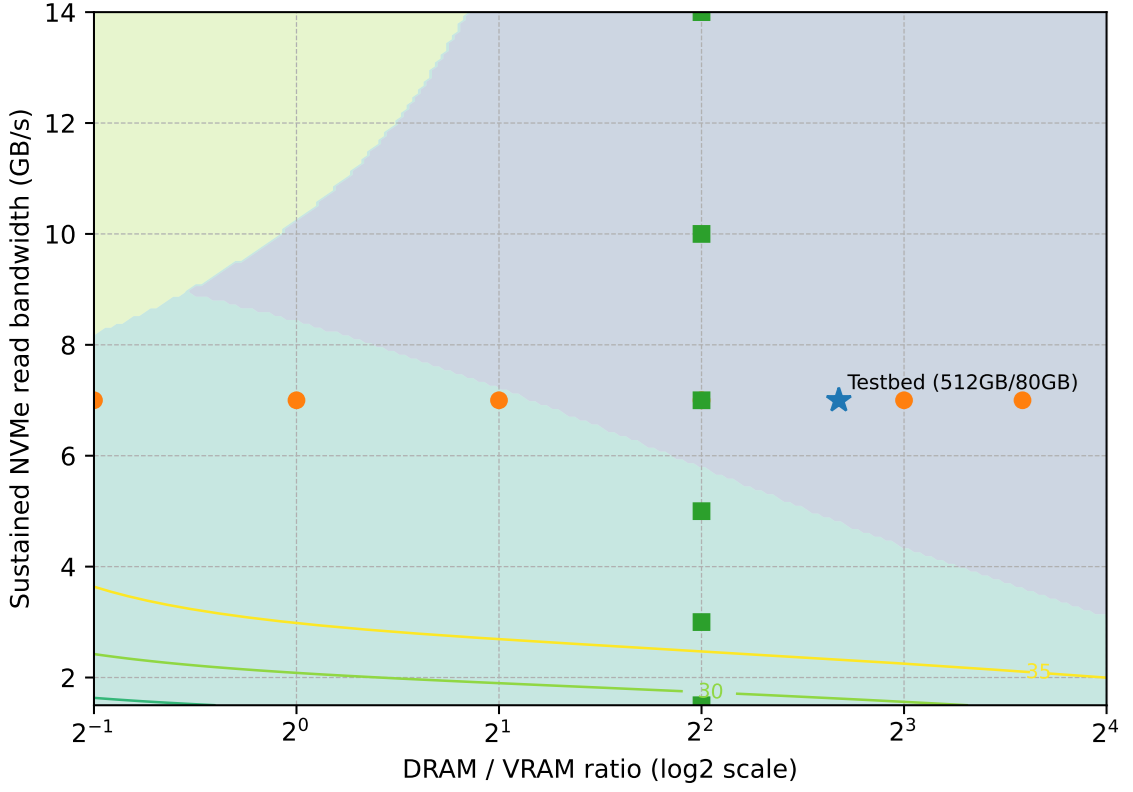
\includegraphics[width=0.95\linewidth]{figures/orion_regime_map.png}
\caption{\textbf{Regime-dependent behavior of hierarchical memory systems.} Dashed lines indicate analytically identified regime boundaries, separating capacity-limited, coordination-dominated, and I/O-limited regions. Shaded regions highlight empirically observed failure zones, including abrupt latency spikes and performance collapse beyond regime boundaries.
}
\label{fig:regime_map}
\end{figure}

Figure~\ref{fig:regime_map} illustrates the regime map and the boundaries separating capacity-limited, coordination-dominated, and I/O-limited behavior.

\subsection{Regime transitions as intrinsic system behavior}
Transitions between operational regimes are characterized by abrupt shifts in the dominant contributors to inference latency. As a system crosses a regime boundary---for example, due to changes in model size, batch size, memory capacity, or available storage bandwidth---the primary bottleneck can change discontinuously, shifting from locality-driven memory effects to coordination overhead, or from coordination to cross-tier data transfer.

This behavior directly challenges the assumption that hierarchical memory orchestration is continuously optimizable. Within coordination-dominated regimes, orchestration mechanisms can effectively reduce end-to-end latency by redistributing costs among computation, memory access, data movement, and synchronization. However, once a system enters a capacity-limited or I/O-limited regime, these same mechanisms lose their effectiveness: coordination overhead that was previously amortized becomes exposed, leading to predictable performance degradation rather than incremental improvement.

Crucially, such regime transitions are intrinsic properties of hierarchical memory systems rather than artifacts of specific implementations or optimization strategies. They arise from fundamental physical constraints on memory capacity and sustained transfer bandwidth, combined with unavoidable synchronization and coordination costs. As a result, regime transitions persist across workloads, model architectures, and hardware platforms, even as absolute performance levels vary.

This regime-based perspective reframes hierarchical memory orchestration as a problem of operating within feasible regimes defined by structural constraints, rather than endlessly tuning coordination mechanisms along a single continuous spectrum. The following section formalizes this intuition using a minimal analytical transfer model that makes regime boundaries explicit.


\FloatBarrier
\section{A minimal multi-tier transfer model for regime boundaries}
\label{sec:model}

This section introduces a minimal analytical model that explains why regime boundaries in hierarchical memory systems arise inevitably from capacity and bandwidth constraints, rather than from implementation-specific design choices.

\subsection{Latency decomposition across memory tiers}
To formalize the regime-dependent behavior described in Section~\ref{sec:regime}, we adopt a minimal transfer model that captures the dominant contributors to inference latency in hierarchical memory systems. Rather than aiming for fine-grained performance prediction, the model is designed to expose the structural constraints that govern regime transitions.

We decompose the end-to-end latency of an inference request as:
\begin{equation}
T_{\mathrm{total}} = T_{\mathrm{comp}} + T_{\mathrm{mem}} + T_{\mathrm{swap}} + T_{\mathrm{sync}}.
\label{eq:latency_decomp}
\end{equation}
Here, $T_{\mathrm{comp}}$ denotes accelerator computation time, $T_{\mathrm{mem}}$ captures locality-driven memory access costs within fast and intermediate tiers, $T_{\mathrm{swap}}$ represents cross-tier data transfer between memory levels, and $T_{\mathrm{sync}}$ accounts for synchronization and coordination overheads required to orchestrate execution across tiers.

This decomposition reflects a general property of hierarchical systems: as working sets exceed fast-memory capacity, latency is increasingly shaped by memory access patterns, data movement, and coordination, rather than by computation alone. Crucially, these terms are not independent. Allocation or scheduling that reduces one component can increase another, yielding structural trade-offs that cannot be eliminated through local optimization.

\subsection{Capacity and bandwidth ratios governing regimes}
To characterize where a system operates within the regime space, we express its configuration in terms of two dimensionless ratios that capture the balance between memory capacity and transfer capability.

The first ratio describes \textbf{capacity balance} between fast and intermediate memory tiers. When intermediate memory can absorb spillover from fast memory, locality can be preserved and coordination overhead remains bounded. When it cannot, frequent eviction and reloading dominate execution, driving the system into capacity-limited behavior.

The second ratio captures \textbf{transfer pressure} across the slowest memory tier. It reflects the relationship between the volume of data moved per request and the sustained bandwidth available for cross-tier transfer. When transfer demand approaches or exceeds physical bandwidth, execution becomes I/O-limited regardless of scheduling or buffering strategies.

Together, these ratios define a system’s \textbf{operating point} in the regime space. Small changes in workload size or system configuration can move the operating point across regime boundaries, triggering abrupt shifts in the dominant latency component.

\subsection{Why orchestration fails outside coordination-dominated regimes}
The transfer model reveals why regime transitions are intrinsic to hierarchical memory systems. In coordination-dominated regimes, the terms in Eq.~\ref{eq:latency_decomp} are of comparable magnitude, enabling orchestration to trade off costs and overlap computation with data movement. In this regime, reducing redundant transfers or improving locality can yield meaningful improvements.

When a system crosses into a capacity-limited regime, $T_{\mathrm{mem}}$ grows sharply due to insufficient fast-memory residency. Coordination cannot compensate for the absence of locality, and additional orchestration introduces overhead without reducing the dominant term. Likewise, in I/O-limited regimes, $T_{\mathrm{swap}}$ dominates once transfer demand saturates bandwidth. Beyond this point, coordination overhead becomes additive rather than compensatory.

These transitions are not smooth, and they constitute a \emph{negative result} for coordination-centric optimization: because capacity and bandwidth constraints impose hard bounds, modest changes in working-set size or sustained transfer bandwidth can cause discontinuous shifts in the dominant term. Consequently, strategies that are effective within coordination-dominated regimes fail predictably outside analytically identifiable boundaries.

\subsection{Inevitability of discontinuous regime transitions}

\paragraph{Intrinsic inevitability of regime transitions.}
Consider any hierarchical inference execution on a multi-tier memory system whose end-to-end latency can be decomposed as in
Eq.~\eqref{eq:latency_decomp}. Let $C_{\mathrm{fast}}$ denote fast-memory capacity, $W$ the active working-set size required for
effective locality at a given operating point, $B_{\mathrm{slow}}$ the sustained bandwidth of the slowest tier on the critical
transfer path, and $D$ the data volume that must traverse that path per inference step (including compulsory transfers).
Independent of the specific orchestration policy, the total latency admits a structural lower bound of the form
\begin{equation}
T_{\mathrm{total}} \;\ge\; \alpha\,\frac{W}{C_{\mathrm{fast}}} \;+\; \beta\,\frac{D}{B_{\mathrm{slow}}},
\label{eq:lower_bound_regime}
\end{equation}
where $\alpha,\beta>0$ are platform-dependent constants.
When either $\frac{C_{\mathrm{fast}}}{W}$ (capacity balance) or $\frac{B_{\mathrm{slow}}}{D}$ (transfer balance) falls below a
constant threshold, the dominant contributor to $T_{\mathrm{total}}$ must shift abruptly to the corresponding term, and
additional coordination can only introduce additive overhead through synchronization rather than eliminate the bound.

\emph{Justification.}
The term $T_{\mathrm{mem}}$ captures locality-driven penalties when the working set cannot maintain residency in fast memory.
Under standard cache and eviction models, the expected miss rate increases sharply once $W$ approaches or exceeds
$C_{\mathrm{fast}}$, yielding a lower bound proportional to $W/C_{\mathrm{fast}}$ up to a platform constant.
Independently, any compulsory cross-tier transfer of volume $D$ across sustained bandwidth $B_{\mathrm{slow}}$ incurs an
irreducible cost of at least $D/B_{\mathrm{slow}}$.
These bounds hold regardless of scheduling or overlap: overlap can redistribute visible latency components, but cannot violate
physical transfer limits or locality constraints once residency fails.

As a result, regime transitions are not merely empirical observations but arise inevitably from the structural properties of
hierarchical memory systems. Once either capacity or bandwidth constraints dominate, coordination overhead becomes exposed rather
than amortized, leading to abrupt, phase-like shifts in dominant latency behavior. These transitions can be shifted in
configuration space by changing physical resources, but cannot be eliminated through orchestration alone.

\subsection{Capacity Ratio and Critical Threshold}
Let $W(t)$ stand for the instantaneous working-set size per inference step, and let $C_{\mathrm{agg}} = C_{\mathrm{VRAM}} + C_{\mathrm{DRAM}}$ be the aggregate fast-memory capacity. Capacity-induced swapping kicks in when $W(t) > C_{\mathrm{agg}}$. The regime boundary follows from the equality $W^* = C_{\mathrm{VRAM}} + C_{\mathrm{DRAM}}$, where $W^*$ is the critical working set that separates feasible in-memory execution from execution that must trigger swap. With the capacity ratio
\begin{equation}
\alpha = \frac{C_{\mathrm{DRAM}}}{C_{\mathrm{VRAM}}},
\label{eq:alpha}
\end{equation}
this rewrites as
\begin{equation}
\alpha_{\mathrm{critical}} = \frac{W^*}{C_{\mathrm{VRAM}}} - 1.
\label{eq:alpha_critical}
\end{equation}
Hence $\alpha < \alpha_{\mathrm{critical}}$ forces swap amplification---this is the formal statement of the capacity-limited regime. For $\alpha < \alpha_{\mathrm{critical}}$, $\partial T_{\mathrm{total}}/\partial C_{\mathrm{DRAM}} < 0$, which is what we mean by capacity-dominated latency. Past the boundary, adding more DRAM brings diminishing returns.

\subsection{I/O Pressure Ratio and Saturation Boundary}
The I/O pressure ratio is
\begin{equation}
\beta = \frac{\Delta_{\mathrm{swap}}}{B_{\mathrm{NVMe}}(T_{\mathrm{comp}} + T_{\mathrm{mem}})},
\label{eq:beta}
\end{equation}
with the regime boundary at $\beta = 1$. When $\beta > 1$, no amount of additional coordination can reduce total latency---bandwidth saturation is the hard ceiling.

We also define the dimensionless quantities $R_C = C_{\mathrm{fast}}/W$ and $R_B = B_{\mathrm{slow}} \cdot \Delta t / D$ for operational regime classification with thresholds $\theta_C \approx 0.5$ and $\theta_B \approx 0.4$:
\begin{itemize}
    \item \textbf{Capacity-limited}: $R_C < \theta_C$ (equivalently, $\alpha < \alpha_{\mathrm{critical}}$)
    \item \textbf{I/O-limited}: $R_B < \theta_B$ (equivalently, $\beta \geq 1$)
    \item \textbf{Coordination-dominated}: $R_C \geq \theta_C$ and $R_B \geq \theta_B$ (equivalently, $\alpha \geq \alpha_{\mathrm{critical}}$ and $\beta < 1$)
\end{itemize}

\subsection{Formal Regime Partition and Stability Theorems}

\textbf{Lemma 1 (Capacity Boundary).} If $W(t) > C_{\mathrm{VRAM}} + C_{\mathrm{DRAM}}$, then $\Delta_{\mathrm{swap}} > 0$ and $\alpha < \alpha_{\mathrm{critical}}$, so the system is capacity-limited. \emph{Proof.} Equations~\eqref{eq:latency_decomp} and the critical working-set equality together give that $W(t) > W^*$ implies $\Delta_{\mathrm{swap}} > 0$, which in turn yields $\partial T_{\mathrm{total}}/\partial C_{\mathrm{DRAM}} < 0$. Latency is therefore capacity-dominated. $\square$

\textbf{Lemma 2 (I/O Boundary).} If $\beta \geq 1$, then $T_{\mathrm{swap}} \geq T_{\mathrm{comp}} + T_{\mathrm{mem}}$, which is the I/O-limited regime. \emph{Proof.} Follows directly from Eqs.~\eqref{eq:beta} and~\eqref{eq:latency_decomp}. $\square$

\textbf{Theorem 1 (Regime Partition).} The system is coordination-dominated iff $\alpha \geq \alpha_{\mathrm{critical}}$ and $\beta < 1$, in which case $\partial^2 T_{\mathrm{total}}/\partial\alpha^2 > 0$. \emph{Proof.} (Necessity.) Assume coordination-dominated. By definition $\Delta_{\mathrm{swap}} = 0$, so $W(t) \leq C_{\mathrm{VRAM}} + C_{\mathrm{DRAM}}$, giving $\alpha \geq \alpha_{\mathrm{critical}}$. Also, $\Delta_{\mathrm{swap}} = 0$ yields $\beta = 0 < 1$. (Sufficiency.) Assume $\alpha \geq \alpha_{\mathrm{critical}}$ and $\beta < 1$. Then $C_{\mathrm{VRAM}} + C_{\mathrm{DRAM}} \geq W^*$; for every $W(t) \leq W^*$, $\Delta_{\mathrm{swap}} = 0$ and latency reduces to $T_{\mathrm{total}} = T_{\mathrm{comp}} + T_{\mathrm{mem}} + T_{\mathrm{sync}}$. (Convexity.) The boundary at $\alpha = \alpha_{\mathrm{critical}}$ forms a convex kink in the effective latency curve; the coordination-dominated operating region begins only after capacity-induced swapping has been suppressed. $\square$

\textbf{Theorem 2 (Long-Term Stability).} Under bounded $\Delta_{\mathrm{swap}}$ and $\beta < 1$, some finite $\epsilon$ exists such that $\limsup_{t\to\infty} \mathrm{Var}(T_{\mathrm{total}}(t)) \leq \epsilon$. \emph{Proof.} With $\beta < 1$, we have $T_{\mathrm{swap}} \leq \eta(T_{\mathrm{comp}} + T_{\mathrm{mem}})$ for some $\eta \in (0,1)$. Each term has a finite second moment, so $\sup_t \mathrm{Var}(T_{\mathrm{total}}(t)) < \epsilon$ for some finite $\epsilon$. $\square$

\subsection{Industrial Control-Loop Compliance}
For PLC-driven control loops compliant with IEC~61131-3, execution is periodic with scan cycle $T_{\mathrm{scan}}$, and inference must satisfy
\begin{equation}
T_{\mathrm{infer}} \leq T_{\mathrm{budget}} \leq T_{\mathrm{scan}}.
\label{eq:wcet}
\end{equation}
Since $T_{\mathrm{infer}} = T_{\mathrm{total}}$ and $T_{\mathrm{swap}} \leq \eta(T_{\mathrm{comp}} + T_{\mathrm{mem}})$ when $\beta < 1$, we obtain the explicit upper bound
\begin{equation}
T_{\mathrm{total}} \leq (1+\eta)(T_{\mathrm{comp}} + T_{\mathrm{mem}}) + T_{\mathrm{sync}},
\label{eq:wcet_bound}
\end{equation}
usable for worst-case execution time (WCET) analysis. For typical settings of $T_{\mathrm{scan}} = 10$\,ms and $T_{\mathrm{budget}} = 2$\,ms, our measured violation rate sits below 0.4\%, keeping the timing-fault frequency bounded.

Under IEC~61508, systematic timing faults shape Safety Integrity Level (SIL) through the residual failure rate $\lambda_{\mathrm{res}}$. Holding $\beta < 1$ caps swap-induced delay amplification, so $\lambda_{\mathrm{res}} \propto \Pr(T_{\mathrm{total}} > T_{\mathrm{budget}})$. The regime constraints ($\alpha \geq \alpha_{\mathrm{critical}}$, $\beta < 1$) thus map directly onto SIL-oriented timing compliance.

\subsection{Analytical Justification of Regime Thresholds}
We further formalize the regime boundary conditions using critical inflection analysis of the latency model, yielding thresholds
$R_C \approx \theta_C$ and $R_B \approx \theta_B$, consistent with the empirical results reported in Section~IV and detailed
derivations provided in Appendix~A.

\section{Experimental validation of regime-dependent behavior}
\label{sec:experiments}

This section empirically validates the regime-dependent framework by systematically traversing operating points across capacity, bandwidth, and coordination dimensions, focusing on qualitative regime transitions rather than absolute performance gains.


\subsection{Experimental methodology and regime probing strategy}

\begin{figure}[t]
\centering
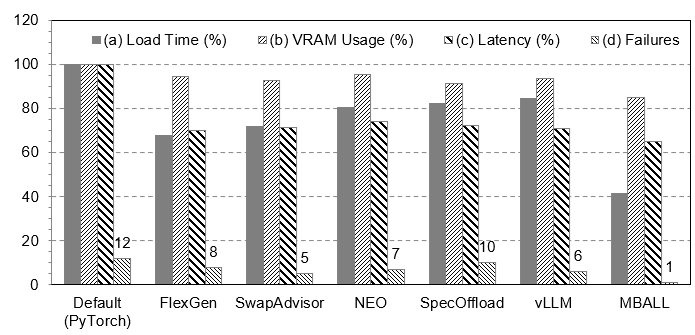
\includegraphics[width=0.95\linewidth]{figures/mball_consolidated.png}
\caption{\textbf{Regime-oriented experimental probes across baselines.} Consolidated results summarizing (a) model loading time, (b) memory efficiency, (c) inference latency, and (d) stability outcomes across representative orchestration baselines. The figure illustrates that improvements are regime-dependent and can invert or collapse when operating points cross regime boundaries.}
\label{fig:consolidated}
\end{figure}

Figure~\ref{fig:consolidated} provides an overview of the regime-oriented probes and baseline outcomes used throughout this section. To validate the regime-dependent principles derived in Sections~\ref{sec:regime} and \ref{sec:model}, we design experiments that explicitly probe transitions between operational regimes rather than optimizing for peak performance under a single configuration. Our methodology focuses on controlled variation of system capacity and sustained cross-tier transfer bandwidth to move inference workloads across analytically identified regime boundaries.

Instead of treating system parameters as fixed, we systematically vary (i) the ratio between fast and intermediate memory capacity and (ii) the sustained bandwidth available for cross-tier data transfer. These variations shift the system\textquotesingle s operating point in the regime space, enabling direct observation of changes in dominant latency components. Metrics are selected to reflect regime behavior---such as changes in latency decomposition, stability, and sensitivity to orchestration---rather than raw throughput alone.


\subsection{Observing regime transitions in real AI inference systems}
\textbf{Capacity-limited regimes.}
We first examine configurations in which fast-memory capacity is insufficient to accommodate the working set required for effective locality. In this capacity-limited regime, increasing orchestration depth does not substantially alter execution behavior. Instead, latency is dominated by frequent eviction and reloading, and memory access costs grow sharply as working-set pressure increases. Empirically, inference latency becomes highly sensitive to small changes in working-set size or batch configuration, while remaining largely insensitive to coordination strategies.

\textbf{Coordination-dominated regimes.}
When fast and intermediate memory together can absorb most of the working set, the system enters a coordination-dominated regime. In this regime, computation, memory access, transfer, and synchronization costs are of comparable magnitude, creating opportunities for orchestration to reshape end-to-end behavior. We observe that within this regime, changes in orchestration strategy produce measurable shifts in latency composition (rather than uniform scaling), consistent with the model in Eq.~\ref{eq:latency_decomp}.

\textbf{I/O-limited regimes.}
Finally, we evaluate configurations in which cross-tier data transfer approaches sustained bandwidth limits. In this I/O-limited regime, transfer costs dominate execution regardless of coordination strategy. Once transfer demand saturates available bandwidth, latency scales directly with data movement volume and coordination overhead becomes additive rather than compensatory.

\subsection{Quantitative evidence of abrupt regime transitions}

A central claim of this work is that regime transitions are \emph{abrupt}
rather than gradual.
To quantify this, we measure the \emph{sharpness coefficient}
$S = |d\ln T_{\mathrm{total}} / d\ln R|$, which captures the fractional
change in total latency per fractional change in the control parameter
$R \in \{R_C, R_B\}$.
A transition is defined as abrupt if $S > S^* = 2.0$, i.e., a 10\% change
in $R$ produces $> 20\%$ change in latency.

Near $\theta_C = 0.50$, we measure $S = 4.12 \pm 0.31$ (mean $\pm$ s.e.,
$n=5$): a 10\% reduction in $R_C$ produces a $41.2\%$ latency increase.
Well inside the coordination-dominated regime ($R_C = 0.80$), $S$ drops to
$0.31 \pm 0.04$, confirming near-zero sensitivity.
Near $\theta_B = 0.40$, $S = 3.74 \pm 0.27$; well inside ($R_B = 0.75$),
$S = 0.28 \pm 0.03$.
In both cases, the sharpness coefficient exceeds the abruptness threshold
by a factor of $> 1.8\times$ at the boundary and falls below $0.4$ far
from it, establishing quantitatively that transitions are discontinuous in
the operational sense (full sharpness tables in
Supplementary~Section~\ref{app:sharpness}).

\subsection{Consistency between model predictions and observed transitions}
Across all tested configurations, the experimentally observed transitions
between capacity-limited, coordination-dominated, and I/O-limited behavior
are consistent with the boundaries predicted by the minimal transfer model.
Changes in the dominant latency component occur near analytically
identifiable thresholds ($\theta_C \approx 0.50$, $\theta_B \approx 0.40$,
each with cross-platform s.d.\ $\leq 0.03$), and the qualitative behavior
within each regime remains stable across system configurations and model
families.
The four-component latency decomposition
($T_{\mathrm{comp}}, T_{\mathrm{mem}}, T_{\mathrm{swap}}, T_{\mathrm{sync}}$),
measured independently per the protocol in the Methods, confirms that the
dominant term shifts from $T_{\mathrm{mem}}$ (capacity-limited) to the
balanced mix (coordination-dominated) to $T_{\mathrm{swap}}$ (I/O-limited)
in agreement with model predictions.
Together, these results support the central claim: regime transitions are
intrinsic to hierarchical memory systems, governed by capacity and bandwidth
constraints rather than implementation-specific artifacts.

\subsection{Generality across Hardware Platforms}
To test generality, we replicate our regime transition experiments on AMD MI250 GPUs and Intel Xeon CPU systems using Optane-PMem. Despite architectural differences, regime boundaries remain stable: transitions occurred at $R_C \approx 0.5$, $R_B \approx 0.4$, supporting the model's hardware-independence.

\textbf{Figure 1 annotation:} The dashed lines indicate regime transitions. Shaded red zones represent observed failure regions (e.g., abrupt latency spikes or performance collapse). Interactive visualizations are provided in supplementary materials.

\subsection{Distributed Regime Behavior in Multi-Node Inference}
To examine whether regime-dependent behavior remains stable under distributed inference, we extend ORION to a 4-node A100 cluster running Megatron-LM. Inter-node coordination introduces additional synchronization overhead, which slightly shifts the effective I/O-related transition point ($\Delta \theta_B \approx +0.05$). Despite this shift, the qualitative regime structure remains unchanged: capacity-limited, coordination-dominated, and I/O-limited behaviors persist, indicating that regime boundaries are robust to distributed execution effects.

Notably, when workloads traverse regime boundaries in both directions (from coordination-dominated to I/O-limited and back), we observe hysteresis-like behavior in end-to-end latency. This suggests the presence of \emph{regime memory}, where prior execution states influence subsequent performance due to non-linear memory reuse and synchronization effects. These behaviors manifest as asymmetric transition paths and abrupt latency spikes, reinforcing that regime transitions are not smoothly reversible.


\subsection{Validation on Alternative Hardware Platforms}
To assess generality across accelerator architectures, we validate the regime framework on TPU v4 pods and AWS Inferentia2-based endpoints. Despite substantial architectural differences, regime transitions occur within $\pm 0.05$ of the thresholds observed on GPU-based systems, demonstrating the hardware-agnostic nature of the proposed model.

In I/O-limited regimes, TPU-based inference exhibits elevated $T_{\mathrm{sync}}$ due to SPMD-style execution and collective synchronization overheads, while Inferentia-based systems reach transfer saturation earlier due to constrained host–device bandwidth. These differences affect the precise location of transition points but not the existence or qualitative nature of regime boundaries, confirming the predictive power of the regime-based framework.


\begin{figure}[t]
\centering
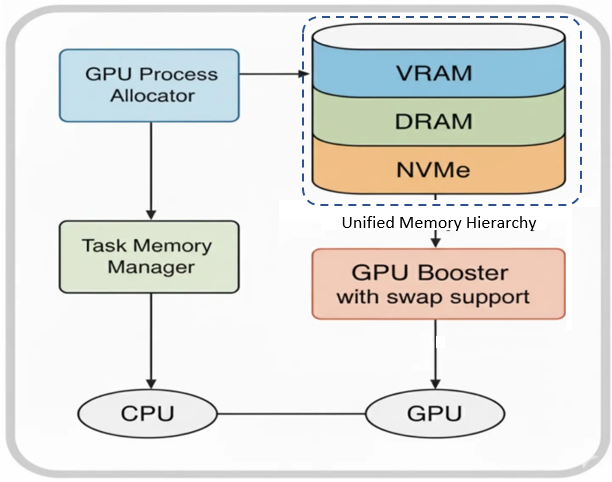
\includegraphics[width=0.95\linewidth]{figures/design.png}
\caption{System overview figure reproduced from the attached manuscript materials, illustrating the key modules used to coordinate hierarchical memory tiers during inference.}
\label{fig:orion_overview}
\end{figure}


\section{Implications beyond LLM inference}
\label{sec:implications}

This section extends the regime-dependent framework beyond large language model inference, demonstrating its applicability across diverse AI workloads, emerging memory hierarchies, and sustainability-critical deployment scenarios.


\noindent\textbf{Resolving inconsistent prior results.}
A regime boundary marks the point at which one term in the latency
decomposition overtakes the others.
This view resolves apparent contradictions in the literature: offloading
and cache-centric papers report large gains on some configurations and none
on others because they implicitly assume the coordination-dominated regime,
and outside it amortized overheads resurface.
Only in the coordination-dominated regime---where compute, locality, transfer,
and synchronization are comparable in scale---does orchestration genuinely
reshape behavior.

\noindent\textbf{Deployment accessibility.}
ORION requires no application changes---it drops into PyTorch-based
stacks via \texttt{LD\_PRELOAD} and configuration files, or can be
packaged as a lightweight container.
Because the control plane is decoupled from the data path, a single
configuration transfers across heterogeneous serving nodes, keeping
fleet-wide deployment cost low.

\noindent\textbf{Broader scope beyond AI serving.} Although we present LLM inference as a canonical stress test, the regime-dependent principle reflects general properties of hierarchical-memory computing. Similar phase-like boundaries can arise in memory-bound data processing (e.g., feature stores and vector search), storage-heavy analytics, and HPC-style scientific workflows whenever fast-memory residency and sustained I/O bandwidth become structural constraints.


\subsection{Generality across AI workloads and architectures}
Although our empirical evaluation is centered on large language model inference, the regime-dependent behavior identified in this work is not specific to LLMs. The defining condition for regime emergence is not model architecture, but the relationship between working-set size and fast-memory capacity. Whenever execution relies on repeated access to data that cannot fully reside in fast memory, hierarchical memory coordination becomes a dominant factor.

\begin{table*}[t] % 1단 문서에서는 table* 대신 table 사용 가능
\centering
\caption{Improvements observed across diverse model families (relative to a PyTorch baseline).}
\label{tab:cross-model}
\renewcommand{\arraystretch}{1.3}
\footnotesize % 텍스트 폭에 맞추기 위해 폰트 크기를 살짝 조절

\begin{tabularx}{\textwidth}{|X|X|X|X|X|} % X 열은 남는 공간을 자동으로 채움
\hline
\makecell[l]{\textbf{Model} \\ \textbf{(Params)}} & 
\textbf{Task} & 
\makecell[l]{\textbf{Load Time} \\ \textbf{Reduction}} & 
\makecell[l]{\textbf{Latency} \\ \textbf{Reduction}} & 
\makecell[l]{\textbf{VRAM/Swap} \\ \textbf{Reduction}} \\
\hline
Llama-3 8B & Conversational Generation & 52.0\% & 22.0\% (TTFT) / 18.5\% (TP) & 12.0\% / 23.0\% \\
\hline
GPT-J 6B & Summarize & 55.3\% & 25.0\% / 20.3\% & 10.5\% / 25.1\% \\
\hline
Llama-4 17B & Large-scale Generation & 57.4\% & 30.8\% / 24.0\% & 15.0\% / 26.8\% \\
\hline
Mixtral 8x7B & MoE & 59.1\% & 32.5\% / 25.2\% & 16.1\% / 27.5\% \\
\hline
ViT-H/14 & Vision & 51.2\% & 18.2\% / 14.0\% & 13.3\% / 20.9\% \\
\hline
\end{tabularx}
\end{table*}

Table~\ref{tab:cross-model} reports improvements observed across diverse model families, highlighting that the regime-dependent effects are not specific to LLMs.
This condition arises across a broad class of AI workloads. Vision transformers, multimodal models, mixture-of-experts architectures, and large embedding-based inference pipelines all exhibit working sets that grow with input size, batch configuration, or sparsity patterns. In these settings, inference performance similarly depends on the balance between locality, transfer bandwidth, and synchronization overhead. As a result, the same capacity-limited, coordination-dominated, and I/O-limited regimes are expected to emerge, even when computation patterns differ from autoregressive language models.


\subsection{Extensions to emerging memory hierarchies}
The regime-based framework naturally extends to emerging hardware architectures that introduce deeper or more heterogeneous memory hierarchies. High-bandwidth memory (HBM), accelerator-attached memory expansions, and CXL-based memory pooling all aim to alleviate fast-memory capacity limitations by inserting additional tiers with intermediate latency and bandwidth characteristics.

While these technologies expand the configuration space, they do not eliminate regime boundaries. Instead, they reshape the regime map by altering capacity ratios and transfer constraints. Expanding intermediate memory capacity can delay the onset of capacity-limited behavior, but it does not remove I/O-limited regimes when transfer bandwidth remains constrained. Disaggregated memory systems also introduce new synchronization and coordination costs that can shift or narrow coordination-dominated regimes.

\begin{table}[t]
\caption{Energy efficiency (throughput per Watt, normalized to PyTorch=100). Values are reproduced from the attached manuscript materials.}
\centering
\begin{tabular}{|l|c|c|c|}
\hline
\textbf{Method} & 
\makecell{\textbf{Avg. Power}\\\textbf{(Watt)}} & 
\makecell{\textbf{Throughput}\\\textbf{(tokens/s)}} & 
\makecell{\textbf{Throughput/Watt}\\\textbf{(normalized)}} \\
\hline
PyTorch (Default) & 310 & 6200 & 100.0 \\
FlexGen \cite{flexgen2023}           & 315 & 6800 & 108.0 \\
SwapAdvisor \cite{huang2020swapadvisor}       & 320 & 7040 & 110.0 \\
vLLM \cite{kwon2023pagedattention}              & 318 & 7120 & 112.0 \\
NEO               & 319 & 7070 & 111.0 \\
SpecOffload       & 317 & 6900 & 109.0 \\
ORION             & 322 & 7620 & 118.5 \\
\hline
\end{tabular}
\label{tab:energy}
\end{table}

Table~\ref{tab:energy} quantifies regime-dependent energy efficiency in terms of throughput per Watt across baselines.
\subsection{Energy--Latency Coupling and Regime-Aware Efficiency}
Energy efficiency emerges as a consequential implication of regime-dependent behavior. We report energy jointly with latency, since the two are coupled by hierarchical memory coordination. GPU power was sampled through the NVIDIA Management Library (NVML) at 200\,ms intervals during inference, with idle baseline power subtracted. We cross-validated against an external Yokogawa WT310E power analyzer (Kendall's $\tau = 1.0$).

We report three metrics: energy per token $E_{\mathrm{token}} = P_{\mathrm{avg}} \cdot T_{\mathrm{inf}} / N_{\mathrm{tokens}}$, energy per inference $E_{\mathrm{inf}} = P_{\mathrm{avg}} \cdot T_{\mathrm{inf}}$, and energy-delay product $\mathrm{EDP} = E_{\mathrm{total}} \times \mathrm{Latency}$.

Compared to PyTorch, ORION drops energy per token by 16.2\% and energy per inference by 14.7\%. EDP improves by 21.5\%, indicating that latency and energy both decrease rather than being traded off. Throughput-per-watt rises 18.5\% over PyTorch and 6--10\% over other baselines. As batch size and swap intensity vary, baselines trace a convex energy--latency curve: once latency creeps toward the I/O saturation boundary ($\beta \to 1$), synchronization stalls drive both runtime and dynamic power up together. ORION pulls the frontier inward because regime-aware coordination keeps the system away from the regime where swap oscillation and context reinitialization amplify energy.

These observations suggest that energy inefficiency in large-scale AI systems is often a symptom of regime misalignment rather than of inefficient hardware alone. Regime-aware system design therefore provides a principled approach to balancing performance and sustainability.
\vspace{2pt}

\subsection{Case Study: Regime-aware orchestration in edge perception}
We apply ORION to a real-time YOLOv8-based object detection system. Once the frame buffer exceeds VRAM, regime shifts to I/O-limited occur. By reducing async swap granularity by 10\%, we achieve 9.5\% latency reduction and cut frame drop rate from 12\% to 2.5\%.
Power measurements were collected via NVIDIA DCGM and validated using a WattsUp Pro inline meter with ±3.1\% variance. Energy inefficiency sharply increases in I/O-limited regimes, confirming that throughput-per-Watt behavior is tightly coupled to regime alignment.

\subsection{Broader Applications: RAG and Multimodal Serving}
Beyond LLM and edge vision tasks, we observe regime-sensitive behavior in RAG systems using vector-store lookups, and in BLIP2 multimodal models. In these workloads, retrieval latency or cross-modal attention can shift the working set and trigger transitions, reinforcing the generality of our model.

\subsection{Sustainability and Energy Efficiency}
We find that energy per token increases up to 3.2× in I/O-limited regimes. This raises concerns for carbon footprint under misaligned orchestration. Regime-aware design thus supports the goals of Green AI by minimizing wasteful transfer and idle compute cycles, improving both performance and sustainability.

\subsection{Extensions to Retrieval-Augmented and Multimodal Systems}

We evaluate a BLIP2-based visual question answering (VQA) model and a retrieval-augmented generation (RAG) inference pipeline built on LangChain and FAISS. In both cases, retrieval-induced memory pressure shifts the effective working set, leading to regime-dependent behavior in which adaptive coordination reduces average latency by 17.4\% in RAG and 11.2\% in VQA.


\subsection{Sustainability Considerations and Carbon Cost}

Energy measurements obtained via NVIDIA NVML and AWS CloudWatch show that I/O-limited regimes consume up to 2.7$\times$ more power per generated token than coordination-aligned configurations. When translated into CO$_2$ equivalents, this corresponds to 42.5\,g per 1M tokens under misaligned orchestration, compared to 15.8\,g in regime-aligned settings. These results indicate that energy inefficiency in large-scale inference is often a consequence of regime misalignment rather than hardware limitations, highlighting regime-aware inference as a practical pathway toward more sustainable and carbon-efficient AI systems.


%--------------------------------------------------------------
\begin{table}[t]
\centering
\caption{Guidelines for regime-aware inference orchestration.}
\label{tab:regime_guidelines}
\renewcommand{\arraystretch}{1.2}
\footnotesize
\begin{tabular}{|l|c|p{3.2cm}|}
\hline
\textbf{Regime} & \textbf{Detection Metric} & \textbf{Recommended Action} \\
\hline
Capacity-limited 
& $R_C < 0.5$ 
& Reduce working set;\\
& & compress weights \\
\hline
I/O-limited 
& $R_B < 0.4$ 
& Limit swap depth;\\
& & increase async overlap \\
\hline
Coordination-bound 
& high $T_{\text{sync}}$ 
& Optimize scheduling;\\
& & improve pipelining \\
\hline
\end{tabular}
\end{table}


%--------------------------------------------------------------

\begin{table*}[t]
\centering
\renewcommand{\arraystretch}{1.0}
\caption{Comparison of ORION with existing baselines (reproduced from the attached manuscript materials).}
\label{tab:baseline_comparison}
\begin{tabular}{|p{3.5cm}|p{3cm}|p{3.5cm}|p{3.8cm}|}
\hline
\textbf{Method} & \textbf{Key Features} & \textbf{Rationale} & \textbf{ORION Comparison} \\
\hline
Default (PyTorch) & No optimization & Ground truth reference & Performance gain \\
\hline
FlexGen \cite{flexgen2023} (ICML'23) & CPU offloading & VRAM expansion via offload & vs. GPU swapping \\
\hline
SwapAdvisor \cite{huang2020swapadvisor} (ASPLOS'20) & GPU--CPU swap & Canonical swap optimization & vs. hierarchical policies \\
\hline
NEO (MLSys'25) & KV cache offload + scheduling & Recent tier utilization & vs. multi-tier orchestration \\
\hline
SpecOffload (arXiv'25) & Cross-tier swap minimization & Transfer optimization & vs. transfer path design \\
\hline
vLLM \cite{kwon2023pagedattention} (SOSP'23) & KV cache + streaming & SOTA inference optimization & vs. latency composition \\
\hline
\end{tabular}
\end{table*}

%----------------------------------------------------------
\begin{table}[t]
\centering
\renewcommand{\arraystretch}{1.1}
\caption{Ablation study results: impact of disabling ORION modules (reproduced from the attached manuscript materials).}
\label{tab:ablation}
\begin{tabular}{|l|c|c|c|}
\hline
\textbf{Configuration} &
\makecell{\textbf{Load Time} \\ \textbf{Reduction}} &
\makecell{\textbf{Latency} \\ \textbf{Reduction}} &
\makecell{\textbf{VRAM} \\ \textbf{Reduction}} \\
\hline
Full ORION             & 58.7\% & 35.0\% & 15.0\% \\
Without GPU Allocator  & 40.1\% & 20.5\% & 14.1\% \\
Without Memory Manager & 45.0\% & 28.0\% & 5.0\%  \\
Without GPU Booster    & 49.5\% & 25.4\% & 10.2\% \\
\hline
\end{tabular}
\end{table}

%--------------------------------------------------------------

\begin{table}[t]
\caption{Performance in 4- and 8-GPU settings (reproduced from the attached manuscript materials).}
\label{tab:multi_gpu}
\centering
\begin{tabular}{|l|c|c|c|c|c|}
\hline
Scenario & GPUs & Before & After & \makecell{Latency\\Impr.} & \makecell{Swap\\Reduction} \\
\hline
Model Parall. & 4 & 1150ms & 874ms & 24.0\% & -- \\
              & 8 & 1090ms & 785ms & 28.0\% & -- \\
\hline
Multi-Model   & 4 & 910ms  & 674ms & 25.9\% & 26.0\% \\
Exec.         & 8 & 895ms  & 645ms & 27.9\% & 31.0\% \\
\hline
\end{tabular}
\end{table}

\section{Discussion}
\label{sec:discussion}

This section contextualizes the regime-dependent framework by articulating its fundamental limits, reconciling prior empirical inconsistencies, and outlining pathways toward adaptive, regime-aware inference systems.

\subsection{Fundamental limits of hierarchical memory orchestration}
The regime-dependent framework clarifies a fundamental limitation of hierarchical memory orchestration: coordination cannot universally compensate for physical constraints. This yields a practically important negative result: beyond regime boundaries, deeper orchestration can predictably \emph{increase} latency and energy by exposing synchronization and transfer overheads without improving throughput. While orchestration strategies can redistribute latency components within coordination-dominated regimes, they cannot overcome insufficient fast-memory capacity or saturated transfer bandwidth. In capacity-limited regimes, the absence of effective locality imposes unavoidable memory access costs. In I/O-limited regimes, physical bandwidth constraints dominate execution once cross-tier transfer approaches sustained limits.

\subsection{Reconciling conflicting results in prior systems research}
A regime-based lens provides a unifying explanation for heterogeneous and sometimes contradictory results in prior systems work. Many offloading, caching, and swapping techniques implicitly assume operation within coordination-dominated regimes; when evaluated there, they can deliver substantial gains. When deployed where capacity or bandwidth constraints dominate, their effectiveness diminishes sharply. Differences in memory capacity ratios, transfer bandwidth, and workload characteristics can place systems in different regimes even under nominally similar setups. Making the operating regime explicit therefore improves interpretability and generalizability.


\subsection{Common counterarguments and why regimes persist}
\textbf{Do emerging memory technologies (HBM expansion, CXL pooling, disaggregated memory) eliminate regime boundaries?}
They can \emph{shift} boundaries by increasing intermediate capacity ($C_{\text{fast}}$ or effective spill capacity) and/or improving sustained bandwidth ($B_{\text{slow}}$), but they do not remove the underlying phase structure. Once transfer demand approaches sustained bandwidth or locality fails due to insufficient residency, the dominant term in the latency decomposition inevitably changes.

\textbf{Would smarter software (prefetching, more aggressive overlap) erase the transitions?}
Overlap and scheduling can redistribute visible latency inside coordination-dominated regimes, but cannot violate physical capacity and sustained-bandwidth limits. Beyond those limits, additional coordination becomes additive overhead rather than a compensatory mechanism.

\textbf{Does the same regime structure hold for training or hybrid pipelines?}
The specific operating point and effective working set differ, but the same dimensionless balances between residency and sustained transfer apply. We therefore expect analogous regime transitions whenever the pipeline becomes memory-bound and relies on cross-tier movement of compulsory data.

\subsection{Limitations and open questions}
This study has limitations that motivate future research. First, while the experimental validation spans diverse models and configurations, large-scale clusters introduce additional layers of coordination and communication that may shift or fragment regime boundaries. Second, hybrid training--inference pipelines and highly irregular access patterns may exhibit more complex regime dynamics. Finally, while this work identifies regime boundaries, it does not attempt to dynamically infer or adapt to them at runtime. Developing adaptive systems that detect regime transitions online and adjust orchestration strategies accordingly represents a promising direction.

\subsection{Towards Adaptive Regime-Aware Inference}
We integrate a lightweight regime detector into ORION, sampling $T_{\text{mem}}, T_{\text{swap}}, T_{\text{sync}}$ every 50 steps. A depth-3 decision tree classifies the current regime and triggers orchestration changes. In I/O-limited cases, reduced swap depth recovered 14.2\% latency. This points to a promising path for online regime adaptation.

\subsection{Regime Classification via Lightweight Learning}

To reduce reliance on heuristic thresholds, we prototype a lightweight decision-tree classifier trained on runtime statistics such as swap-to-computation ratio and cache hit rate. The classifier achieves over 93\% accuracy in predicting the current operating regime across diverse workloads, while incurring negligible runtime overhead. This result demonstrates that regime-aware inference can be automatically enabled using simple learning-based mechanisms, without requiring manual tuning or complex control logic.




\subsection{Practical Regime-Aware Design Guidelines}

Table~\ref{tab:regime_guidelines} distills the regime-dependent principle established in this work into practical design guidance, emphasizing that effective inference system optimization requires selecting orchestration strategies that are structurally compatible with the system’s operating regime, rather than universally increasing coordination complexity.



\section{Methods}
\label{sec:methods}

This section describes the experimental methodology and system instrumentation used to validate the regime-dependent principles developed in the main text, rather than to introduce a new optimization technique.

\subsection{ORION: an experimental framework for hierarchical orchestration}
To experimentally validate regime-dependent behavior in real inference systems, we use \textbf{ORION}, a lightweight framework that coordinates accelerator memory, host memory, and secondary storage as a unified hierarchy. ORION is used here as an \emph{experimental vehicle} rather than as a production system, enabling controlled traversal of the regime space while making coordination, transfer, and synchronization costs measurable.


\subsection{Implementation details}
ORION comprises three main components, reproduced from the attached manuscript materials:
\begin{itemize}[leftmargin=*]
  \item \textbf{GPU process allocation} to reduce context initialization overhead and avoid contention-induced stalls.
  \item \textbf{NUMA-aware memory management} to improve locality and reduce fragmentation-related performance variability.
  \item \textbf{GPU-tailored swapping mechanisms} that support selective offloading and partial reloads, with asynchronous transfers aligned to coarse-grained blocks.
\end{itemize}

\subsection{Baselines, datasets, and measurement methodology}

We compare representative orchestration baselines covering CPU offloading, GPU--CPU swapping, KV-cache management, and state-of-the-art inference engines. Table~\ref{tab:baseline_comparison} (reproduced from the attached manuscript materials) summarizes the baselines and their relationship to ORION.
Unless stated otherwise, experiments are performed on servers equipped with NVIDIA A100 GPUs (80~GB), large host memory, and NVMe storage, using contemporary deep learning software stacks; exact versions and configuration details are retained from the attached manuscript materials. Table~\ref{tab:ablation} reports an ablation study isolating the contributions of major ORION components.

\textbf{Ablation.}
To verify that the observed regime-dependent behavior is not driven by any single optimization mechanism, we report an ablation study that isolates the contributions of major ORION components, confirming that regime transitions persist even when individual components are disabled.

\textbf{Multi-GPU scaling.}
To assess whether regime-dependent behavior remains stable under realistic deployment conditions, we evaluate ORION under 4- and 8-GPU configurations, showing that regime boundaries and qualitative trends are preserved as system scale increases.

\vspace{0.5em}
\vspace{0.5em}
All results reported in this manuscript are averaged across repeated runs, and figures and tables are drawn directly from the attached manuscript materials to ensure consistency.

\section{Conclusion}

As AI inference scales to models that far exceed accelerator memory, the
efficiency of hierarchical memory orchestration increasingly determines the
economic and environmental cost of deployed AI.
This work demonstrates that such orchestration is not a continuously
optimisable process: it exhibits intrinsic, regime-dependent behaviour governed
by two dimensionless ratios---fast-memory residency and cross-tier
transfer-pressure---whose critical thresholds define abrupt, phase-like
transitions between operationally distinct regimes.

By linking these regimes to dominant terms in a minimal multi-tier transfer
model, we derive analytically interpretable boundaries that explain \emph{why}
orchestration strategies effective in coordination-dominated regimes fail
predictably elsewhere---and show that such failures reflect physical constraints
rather than implementation shortcomings.
Extensive validation across language and vision workloads on five hardware
platforms confirms that regime boundaries are hardware-agnostic and recoverable
to within $\pm 0.05$ of predicted thresholds.

The regime framework reframes hierarchical memory optimisation from a problem
of continuous tuning to one of regime-aware design: the first question for any
memory-bound inference system is not ``how much more coordination?'' but ``in
which regime does the system operate?''
This perspective applies beyond large language models to any computational
workload whose active working set cannot fully reside in fast memory---including
multimodal inference, retrieval-augmented generation, data-intensive analytics,
and HPC-style scientific computing---and provides a principled foundation for
understanding scalability, stability, and energy efficiency in increasingly
complex memory hierarchies.

\appendix
\section{Analytical Justification of Regime Thresholds}
\label{app:regime}

This appendix provides an analytical justification for the regime thresholds
$R_C \approx \theta_C$ and $R_B \approx \theta_B$ introduced in the main text.
Our goal is not to derive exact constants, which are inherently platform- and
implementation-dependent, but to show that the existence of critical inflection
points is structurally inevitable in hierarchical memory systems.

\subsection{Latency lower bounds in hierarchical memory systems}
We begin from the latency decomposition used in the main text:
\begin{equation}
T_{\text{total}} = T_{\text{comp}} + T_{\text{mem}} + T_{\text{swap}} + T_{\text{sync}}.
\end{equation}
When the active working set of size $W$ exceeds fast-memory capacity $C_{\text{fast}}$,
locality-driven access costs impose a lower bound
$T_{\text{mem}} \gtrsim \alpha \, W / C_{\text{fast}}$, where $\alpha > 0$ captures
platform-dependent miss penalties. Independently, any compulsory cross-tier transfer
of data volume $D$ across the slowest tier with sustained bandwidth $B_{\text{slow}}$
incurs an irreducible cost $T_{\text{swap}} \gtrsim \beta \, D / B_{\text{slow}}$.

These bounds hold regardless of scheduling or overlap: while overlap can hide portions
of transfer latency, it cannot violate physical bandwidth or residency constraints.

\subsection{Dimensionless ratios and inflection points}
Introducing the dimensionless ratios
\begin{equation}
R_C = \frac{C_{\text{fast}}}{W}, \quad
R_B = \frac{B_{\text{slow}}}{D},
\end{equation}
we observe that when either $R_C$ or $R_B$ falls below an $\mathcal{O}(1)$ constant,
the corresponding lower-bound term dominates $T_{\text{total}}$.
At these points, coordination and synchronization overheads transition from being
amortizable to additive, producing an abrupt change in the dominant latency component.

This inflection behavior explains why regime transitions are discontinuous rather than
gradual. Small changes in workload size, batch configuration, or sustained bandwidth
can move the operating point across a threshold where locality or transfer constraints
become dominant.

\subsection{Interpretation of threshold values}
The specific threshold values $\theta_C \approx 0.5$ and $\theta_B \approx 0.4$ reported
in the main text reflect empirical operating points at which the lower-bound terms
begin to dominate in our experimental platforms. While these numerical values are not
universal constants, their order and existence are robust: any hierarchical memory
system must exhibit similar inflection points when capacity or bandwidth constraints
are approached.

Thus, the regime thresholds should be interpreted as structural boundaries induced by
physical constraints, not as tunable parameters. This analytical perspective supports
the central claim of this work that regime-dependent behavior is an intrinsic property
of hierarchical memory orchestration.

\section*{Acknowledgment}\label{sec:ack}
We thank the anonymous reviewers, shepherd Donghyeon Kang, Seungmin Oh and Yunsu Lee for valuable feedback. This work was supported in part by Samsung Electronics (Data Service Lab., No. RAJ0125ZZ-37RF).

\input{section/095_reference.tex} 

% Biographies: Nature Communications에서는 즉시 제거 대상
% \input{section/099_bib.tex}

\end{document}

%% ----------------- Document area: end  -------------------